\documentclass[border=2pt]{standalone}
\usepackage{tikz,amsmath}
\begin{document}
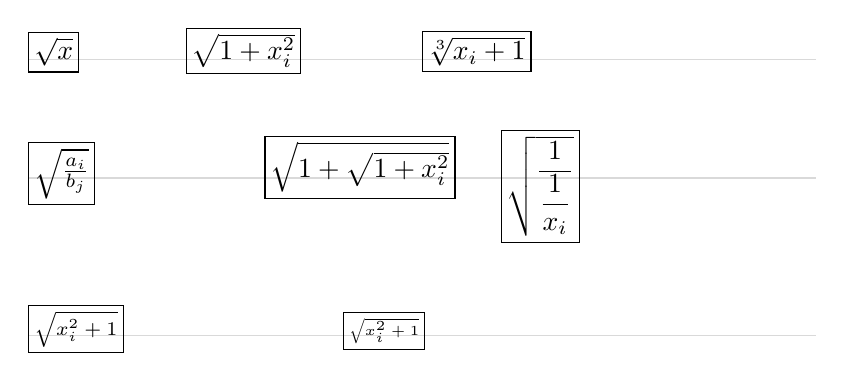
\begin{tikzpicture}
  \draw[gray!30] (0,0)--(10,0) (0,-1.5)--(10,-1.5) (0,-3.5)--(10,-3.5);
  \node[anchor=base west,draw,inner sep=2pt] at (0,0) {$\sqrt{x}$};
  \node[anchor=base west,draw,inner sep=2pt] at (2,0) {$\sqrt{1+x_i^2}$};
  \node[anchor=base west,draw,inner sep=2pt] at (5,0) {$\sqrt[3]{x_i+1}$};
  \node[anchor=base west,draw,inner sep=2pt] at (0,-1.5) {$\sqrt{\frac{a_i}{b_j}}$};
  \node[anchor=base west,draw,inner sep=2pt] at (3,-1.5) {$\sqrt{1+\sqrt{1+x_i^2}}$};
  \node[anchor=base west,draw,inner sep=2pt] at (6,-1.5) {$\sqrt{\dfrac{1}{\dfrac{1}{x_i}}}$};
  \node[anchor=base west,draw,inner sep=2pt,font=\scriptsize] at (0,-3.5) {$\sqrt{x_i^2+1}$};
  \node[anchor=base west,draw,inner sep=2pt,font=\tiny] at (4,-3.5) {$\sqrt{x_i^2+1}$};
\end{tikzpicture}
\end{document}
